\renewcommand{\lecturetitle}{NAS-Bench-101: The first NAS benchmark}
\renewcommand{\lecturetime}{Week 9, Video 4}
\section{\lecturetitle}
%-------------------------------------------------
%-------------------------------------------------

%----------------------------------------------------------------------
\myframe{Blackbox NAS Methods on NAS-Bench-101 \litw{\href{http://proceedings.mlr.press/v97/ying19a.html}{Ying et al, 2018}}}{
	\myit{
%		\item All methods find good architectures
		\item RL outperforms random search
		\item BO and regularized evolution perform best, better than RL
	}
	\centering
	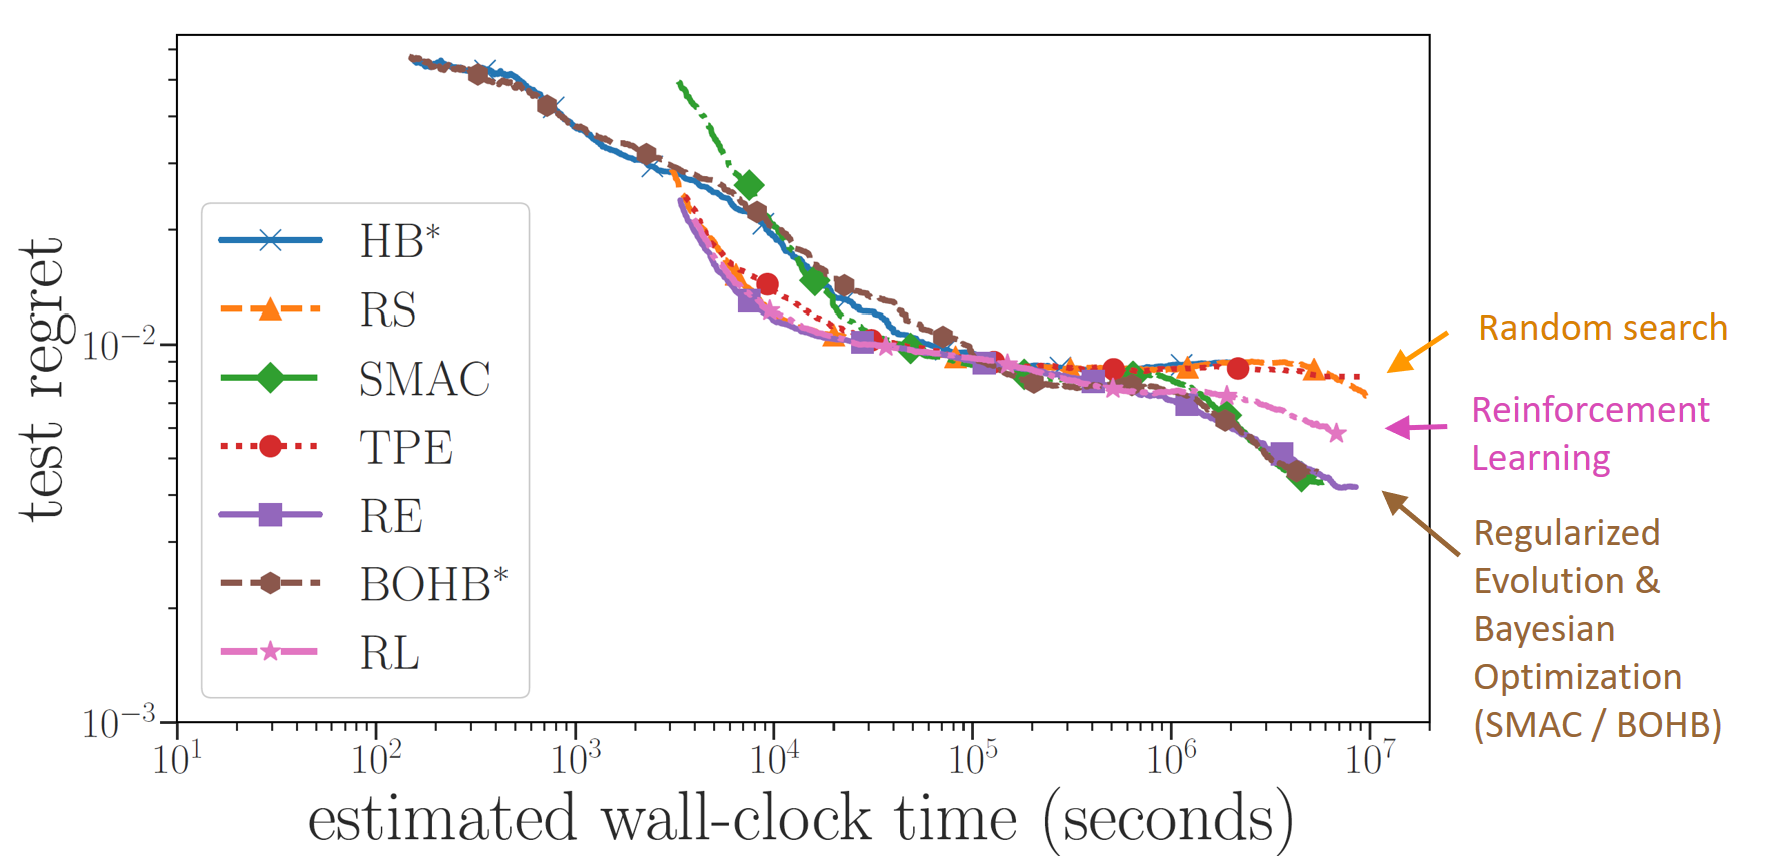
\includegraphics[width=.7\textwidth]{images/NAS-Bench-101-results-with-labels}

\pause
	\myit{
		\item Note that the BO method SMAC \lit{\href{https://link.springer.com/chapter/10.1007/978-3-642-25566-3_40}{Hutter et al, 2011}} \\
		predated RL for NAS \lit{Zoph \& Le, 2017} by 6 years
		\myit{
			\item[-] Only now, benchmarks like NAS-Bench-101 allow for efficient comparisons
		}
	}
}
%-----------------------------------------------------------------------

%----------------------------------------------------------------------
\myframe{Questions to Answer for Yourself / Discuss with Friends}{

	\myit{
		\item Repetition: \alert{Which blackbox NAS approach popularized the field?}
\medskip
		\item Repetition: \alert{Which blackbox NAS approach works best (to date)?}
\medskip
		\item Discussion: \alert{Given enough resources, will blackbox NAS approaches always improve performance?}
	}
}
%-----------------------------------------------------------------------
